\documentclass[10pt, a4paper]{article}
\usepackage[utf8]{inputenc}
\usepackage{pdflscape}
\usepackage[french]{babel}
\usepackage{amssymb}
% \usepackage[margin=3cm]{geometry}
\usepackage{graphicx}
\usepackage{oz}
\usepackage{array,multirow,makecell}
\setcellgapes{1pt}
\usepackage[top=4cm,bottom=4cm,left=3cm,right=3cm]{geometry} %marges
\newcolumntype{R}[1]{>{\raggedleft\arraybackslash }b{#1}}
\newcolumntype{L}[1]{>{\raggedright\arraybackslash }b{#1}}
\newcolumntype{C}[1]{>{\centering\arraybackslash }b{#1}}

\title{Analyse Projet BDD}
\date{}
\begin{document}


\maketitle
\tableofcontents
\newpage

\section{Analyse du problème}
\subsection{Hypothèses}
Pour la conception, nous avons fait les choix suivants:
\begin{enumerate}
    \item Le statut des commandes n'est pas dans l'entité mère COMMANDES
          mais dans ses sous-entités afin d'éviter d'avoir des statuts non cohérents
          pour un type de commande donné.
    \item Nous avons rajouté le statut ``terminée'' qui indique qu'une
          commande a effectivement été effectuée et que l'on peut donner un
          évaluation.
    \item Nous avons choisi, lorsque le client fait appel au droit à l'oubli de ne pas lui créer de nouvel identifiant car il en possède déjà
          un qui est uniquement vu par la base de données et auquel il n'a pas accès. Cette modification n'aurait donc était qu'une modification de nombreuses tables.
    \item Concernant les statuts des commandes, nous supposons que ce sont les restaurants qui s'occupent d'actualiser dans la base de données leur commande.
    \item Pour les catégories, nous avons ajouté une catégorie mère '\_' qui est la racine des catégories.
\end{enumerate}

\subsection{Exemple du passage de l'énoncé aux contraintes : cas des plats}
L'énoncé donnait la portion suivante sur les plats:
\\

\textit{``Un plat est identifié par un \textbf{numéro unique au restaurant} qui le propose et possède \textbf{un nom}, \textbf{une description},
\textbf{un prix} et \textbf{optionnellement une liste des allergènes} qu’il peut contenir.''}
\\

On obtient donc l'entité \textbf{Plats} et les attributs \{\underline{Pid, PRestaurant}, PNom, Description, PPrix, PAllergenes \}.
De cette phrase on en déduit: 
\\ 

La DF: (PId, Restaurant) \(\rightarrow \) PNom, PDescription, PPrix
\\

La contrainte de valeur: PPrix \(>\) 0
\\

La contrainte de multiplicité: (PId, RMail) \(\psur \) ANom


\begin{landscape}
    \subsection{Contraintes}

    Après analyse du texte, nous avons relevé les contraintes suivantes:

    \begin{center}
        \[
            \begin{tabular}{|C{5cm}|C{5cm}|C{5cm}|C{5cm} |}

                \hline
                DF                                                                              & C. Valeurs
                                                                                                & C. Contextuelles                                                           & C. Multiplicité                                                          \\
                \hline

                RMail $\rightarrow$ RNom, RNumero, RAdresse, Places,
                Presentation, RNote                                                             & RType $\in$ \{livraison, emporter, place\}                                 & $\sum
                    \mbox{nbPers}  \le \mbox{Places} $ pour un restaurant et ses commandes
                associées                                                                       & RMail $\twoheadrightarrow$ JourPlage                                                                                                                  \\

                                                                                                & Places $> 0$                                                               & $\mbox{Ext(CEId)} \cap \mbox{Ext(CPId)} \cap
                \mbox{Ext(CLId)} = \emptyset $                                                  & RMail  $\twoheadrightarrow$
                TypeCommande                                                                                                                                                                                                                            \\

                                                                                                & RNote $\in  [0,5] $                                                        & $\mbox{Ext(CEId)} \cup \mbox{Ext(CPId)} \cup
                \mbox{Ext(CLId)} = \mbox{Ext(CId)}$                                             & RMail $\twoheadrightarrow$ PId                                                                                                                        \\
                \cline{1-2}

                (PId, Restaurant) $\rightarrow$ PNom, PDescription, PPrix                       & PPrix $>0$                                                                 &
                CPArrivee $\in$ JourPlage pour un restaurant et ses commandes associées         &
                RMail $\twoheadrightarrow$ CatNom                                                                                                                                                                                                       \\
                \cline{1-2}

                U\_Id $\rightarrow$ UMail, UMdp, UNom, UPrenom, UAdresse                        &                                                                            & CDate donne JourPlage pour toute commande    & (PId, RMail) $\psur$ ANom \\
                \cline{1-2}

                CId $\rightarrow$ CDate, CPrix                                                  & CPrix $>0$                                                                 & CDate $<$ EDate                              &
                CId $\twoheadrightarrow$ (PId, RMail)                                                                                                                                                                                                   \\
                \cline{1-2}

                CLId $\rightarrow$ CLAdresse, Indications, CLArrivee, CLStatut                  &
                CLStatut $\in$ \{ attente, validée, en livraison, annuleeC, annuleeR,
                terminee \}                                                                     &
                EId $\Rightarrow$ CId.statut = \{terminee\}
                                                                                                & CId $\rightarrow$ TypeCommande                                                                                                                        \\
                \cline{1-2}

                CEId $\rightarrow$ CEStatut                                                     &
                CEStatut $\in$ \{ attente, validée, disponible, annuleeC, annuleeR, terminee \} & CDate $\geq$ DateActuelle                                                  & CId $\rightarrow$ U\_Id                                                  \\
                \cline{1-2}

                CPId $\rightarrow$ NbPers, CPArrivee, CPStatut                                  &
                CPStatut $\in$ \{ attente, validée, annuleeC, annuleeR,
                terminee \}                                                                     & CPArrivee $\geq$ DateActuelle                                              & CId $\pfun$
                EId                                                                                                                                                                                                                                     \\

                                                                                                & NbPers $>0$                                                                &                                              & CatNom $\pfun$ CatNom     \\
                \cline{1-2}

                EId $ \rightarrow$ EDate, Avis, ENote                                           & ENote $ \in [0..5] $                                                       &
                EDate $\geq$ DateActuelle                                                       &                                                                                                                                                       \\
                \cline{1-2}

                                                                                                & JourPlage $\in $ \{LM, LS, MaM, MaS, MeM, MeS, JM, JS, VM, VS, SM, SS, DM,
                DS \}                                                                           & CType $\in$ TypeCommande pour un CId donné et le RMail associé             &                                                                          \\
                \hline
            \end{tabular}
        \]
    \end{center}


    \newpage
    \subsection{Diagramme Entités/Associations}
    On obtient ensuite le diagramme Entité/Associations suivant (à noter qu'une légende est présente puisque nous n'avons pas utilisé le même formalisme que celui du cours avec le logiciel utilisé):
    \begin{center}
        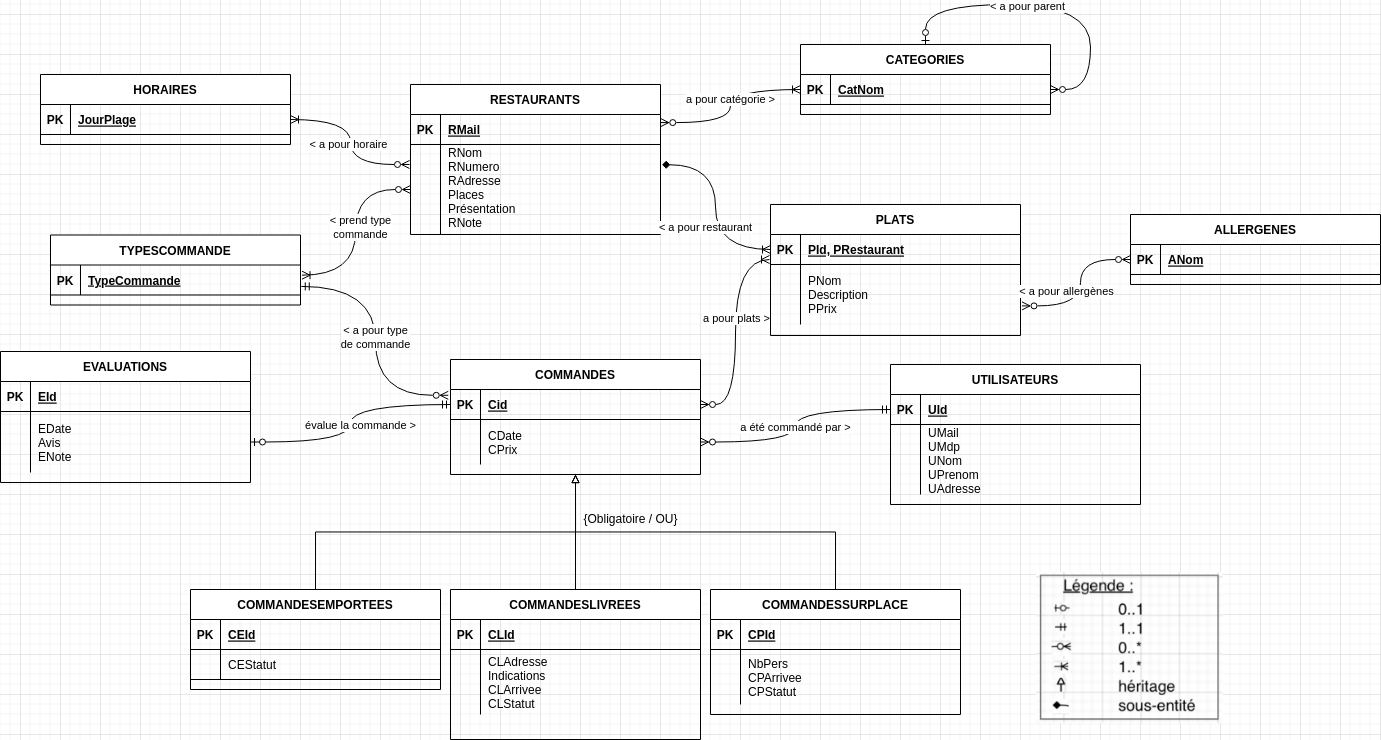
\includegraphics[scale=0.45]{Diagramme_entite_relation.png}\\
    \end{center}

\end{landscape}

Quelques précisions sont à apporter:

\begin{itemize}
    \item Pour une question d'espace occupé nous avons décidé de traduire l'héritage des différentes catégories des commandes par référence. Contrairement à l'unification cela nous permet de ne pas avoir à gérer les contraintes avec l'application. Cependant, cela nous force à faire des jointures lorsque l'on souhaite accéder à toutes les données.
    \item L'héritage que l'on fait pour les différents types de commandes est dans le cas d'une contrainte de partition: celui-ci doit être obligatoire, et une commande ne peut pas à la fois être à emporter et sur place par exemple.
    \item La cardinalité de la flèche allant de la table ALLERGENES à PLATS est de 0..* puisque nous avons fait le choix (cf. partie sur le peuplement) de remplir cette première table de manière exhaustive avec tout les allergènes alimentaires définis par le règlement UE. Ce choix a été fait car la liste complète ne prend pas beaucoup de place dans la base de données.

\end{itemize}

\section{Modèle Relationnel}

Nous avons appliqué l'algorithme vu en cours pour obtenir le schéma relationnel.

\subsection{Traduction des entités simples}

Nous avons identifié les entités simples suivantes:

\begin{itemize}
    \item RESTAURANTS\@(\underline{RMail}, RNom, RNum, RAdresse, Places, Présentation, RNote)
    \item COMMANDES\@(\underline{Cid}, CDate, CPrix, \textbf{Uid}, \textbf{TypeCommande})
    \item UTILISATEURS\@(\underline{U\_id}, UMail, UMdp, UNom, UPrenom, UAdresse)
    \item EVALUATIONS\@(\underline{Eid}, EDate, Avis, ENote, \textbf{Cid})
    \item HORAIRES\@(\underline{JourPlage})
    \item TYPESCOMMANDE\@(\underline{TypeCommande})
    \item CATEGORIES\@(\underline{CatNom})
    \item ALLERGENES\@(\underline{ANom})
\end{itemize}

\subsection{Sous-types d'entités}

\begin{itemize}
    \item COMMANDESEMPORTEES\@(\underline{CEid}, CEStatut)
    \item COMMANDESLIVREES\@(\underline{CLid}, CLAdresse, Indications, CLArrivee, CLStatut)
    \item COMMANDESSURPLACE\@(\underline{CPid}, NbPers, CPArrivee, CPStatut)
\end{itemize}

\subsection{Type d'entité faible}

\begin{itemize}
    \item PLATS\@(Pid, PRestaurant, PNom, Description, PPrix)
\end{itemize}

\textbf{Contrainte induite par la traduction}: Vérifier que tout restaurant a au moins un plat.

\subsection{Types d'associations}

\subsubsection{Cardinalité 1..1}

Les attributs en gras dans les relations de la partie 2.1 correspondent aux traductions des associations avec cardinalité 1..1.
Aucune vérification supplémentaire n'est à faire puisque la cardinalité dans l'autre sens est de 0 à soit 1 soit plus l'infini.
\subsubsection{Cardinalité 0..1}

\begin{itemize}
    \item CATEGORIEPARENT\@(\underline{CatNom, CatNomMere})
\end{itemize}

\subsubsection{Cardinalité ?..*}

\begin{itemize}
    \item HORAIRESRESTAURANT\@(\underline{RMail, JourPlage})\\
          \textbf{Contrainte induite}: Vérifier qu'un restaurant a au moins un horaire.
    \item CATEGORIESRESTAURANT\@(\underline{RMail, CatNom})\\
          \textbf{Contrainte induite}: Vérifier qu'un restaurant a au moins une catégorie
    \item TYPESRESTAURANT\@(\underline{RMail, TypeCommande})\\
          \textbf{Contrainte induite}: Vérifier qu'un restaurant a au moins un type de commande.
    \item PLATSCOMMANDE\@(\underline{Cid, Pid, PRestaurant}, NbPlats\footnote[1]{Choix de conception fait en aval du passage en relationnel afin de permettre la sélection d'un même plat plusieurs fois dans une commande donnée.})\\
          \textbf{Contrainte induite}: Vérifier qu'une commande a au moins un plat.
    \item ALLERGENESPLAT\@(\underline{Pid, PRestaurant, ANom})
\end{itemize}

Après vérification, toutes les relations sont 3FNBCK exceptées celles qui peuvent contenir des attributs NULL, c'est à dire la table UTILISATEURS\footnote[2]{Nous y reviendrons dans la partie 5 de ce rapport.} ainsi que la table COMMANDESLIVREES qui contient l'attribut CLArrivee qui est NULL tant que la commande n'est pas livrée, puis contenant la date et l'heure de livraison une fois celle-ci effectuée.

\section{Peuplement de la base de données}

Quelques chiffres concernant le peuplement de la base de données:

\begin{itemize}
    \item 100 utilisateurs différents ont été créé dans la table UTILISATEURS.
    \item 19 restaurants différents ont été créé dans la table RESTAURANTS.
    \item 47 plats différents répartis dans ces restaurants ont été créé dans la table PLATS.
\end{itemize}
Les tables à entrées constantes ont été remplies comme suit:
\begin{itemize}
    \item HORAIRES = [LM, LS, MaM, MaS, MeM, MeS, JM, JS, VM, VS, SM, SS, DM, DS]\footnote[3]{Cela correspond à des plages horaires, LM signifiant Lundi Midi par exemple.}
    \item ALLERGENES = [Gluten, Crustacés, Oeufs, Poissons, Arachides, Soja, Lait, Fruits a coques, Céleri, Moutarde, Graines de sésame, Anhydre sulfureux et sulfites, Lupin, Mollusques]
    \item TYPESCOMMANDE = [emporter, place, livraison]
\end{itemize}
\newpage 
La table CATEGORIES a été remplie comme suit:
\begin{center}
    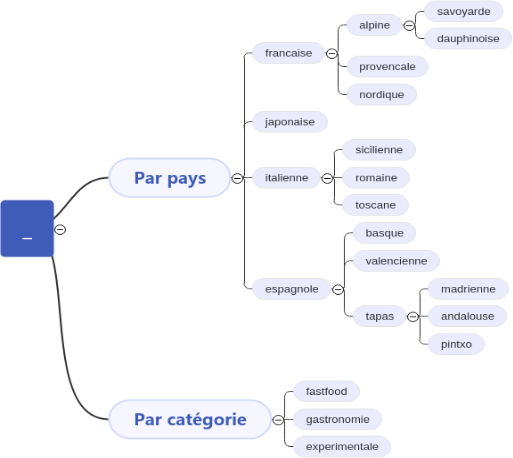
\includegraphics[scale=2.5]{categories.png}
\end{center}

Enfin, les tables faisant le lien entre différentes tables (CATEGORIEPARENT, HORAIRESRESTAURANT, CATEGORIESRESTAURANT, TYPESRESTAURANT, PLATSCOMMANDE et ALLERGENESPLAT) ont été remplies de manière logique en fonction des données rentrées au-dessus.

\section{Analyse des fonctionnalités}
\subsection{Parcours des restaurants}

D'abord, un utilisateur doit pouvoir s'identifier avec son mail et son mot de passe (mdp):

\[
    \pi_{U\_id}(\sigma_{UMail='mail', UMdp='mdp'}(UTILISATEURS))
\]

Il s'agit maintenant de trouver les catégories recommandées en fonction de l'U\_Id préalablement enregistré d'un utilisateur. Ici, nous avons considéré les catégories non pas les plus utilisées par un utilisateur mais seulement les dernières catégories commandées par celui-ci. Il conviendrait de demander au client quel type de recommandation il préfère.

\[
    \pi_{CatNom}(\sigma_{COMMANDES.U\_Id = U\_Id}(CATEGORIESRESTAURANT \Join RESTAURANTS \\ \Join_{PRestaurant = RMail} PLATSCOMMANDE \Join COMMANDES))
\]

Les résultats pourront ensuite être triés par date de commande de la plus récente à la plus ancienne, et limiter le nombre de résultats par exemple aux 5 dernières catégories.
\\

Sinon, il s'agit de parcourir les catégories à la façon d'un menu déroulant, en partant de la racine jusqu'à une catégorie fille souhaitée, par exemple:

\[
    \pi_{CatNom}(\sigma_{CatNomMere='\_'}(CATEGORIEPARENT)) \\
\]

puis

\[
    \pi_{CatNom}(\sigma_{CatNomMere='Par\ pays'}(CATEGORIEPARENT))
\]
on veut par exemple sélectionner les restaurants de cuisine française qui sont ouverts les mardi midi (JourPlage = 'MaM'):

\[
    \pi_{attr}(\sigma_{P}(CATEGORIESRESTAURANT \Join RESTAURANTS \Join HORAIRESRESTAURANT))
\]

Avec \(attr = \) (RMail, RNom, Presentation, RNum, RAdresse, Place, Note) et \\ \(P =\ \)(CatNom='francaise', JourPlage='MaM')
\\

À noter qu'à la différence du démonstrateur, ici, on passe par la description complète des restaurants trouvés avant d'en sélectionner un pour commander.

\subsection{Droit à l'oubli}
Le droit à l'oubli modifie uniquement la table utilisateur mais n'est pas exprimable
avec l'algèbre relationnel. Pour un utilisateur, identifié de manière secrète par son U\_Id, le droit à l'oubli remplacera toutes ses informations par des NULL\footnote[1]{Comme dit précédemment, nous y reviendrons dans la partie 5} tout en conservant son U\_Id.

\subsection{Passage de commande}
Pour le passage de la commande, il y a plusieurs requêtes nécessaires.
Les premières étapes:
\begin{itemize}
    \item Insertion de la commande
    \item Ajout des plats
    \item Ajout du type de la commande
\end{itemize}
ne seront pas exprimables avec l'algèbre relationnel car il s'agit de modifier les tables.
On peut toutefois récupérer les tuples (PPrix, NbPlats) qui vont servir à calculer le coût total pour une commande de Cid = $Cid_0$:
$$
    \pi_{PPrix, NbPlats}( \sigma_{Cid = Cid_0}(PLATS \Join PLATSCOMMANDE))
$$
De même, il est possible d'avoir le nombre de personnes sur place pour toutes les commandes sur place passées pour un horaire demandé = $time$ et un restaurant = $restaurant$ :

$$
    \pi_{Cid, NbPers}(\sigma_{CPArrivee - time < '4h'}(COMMANDES \Join_{CType = 'sur place'} COMMANDESSURPLACE
    $$

    $$
    \Join_{PRestaurant = 'restaurant'} PLATSCOMMANDE))
$$
On remarquera que dès que plusieurs plats auront été commandés pour une même commande, on aura alors
une répétition qu'il faudra donc trier avec l'API.

\newpage

\section{Fonctionnalités manquantes et améliorations}

Il reste encore beaucoup de points que nous n'avons pas eu le temps de faire et quelques améliorations que nous pouvons d'ores et déjà pointées:

\begin{itemize}
    \item L'application Java ne vérifie pas que les horaires d'un restaurant sont compatibles avec les commandes des utilisateurs.
    \item De ce fait, il n'y a pas non plus la possibilité de filtrer les restaurants en fonction de leurs horaires d'ouverture, comme demandé dans la partie des fonctionnalités.
    \item De même, il n'y a pas de vérification en terme de type de commande passée par un utilisateur à un restaurant. Ainsi, il est possible de demander une livraison à un restaurant ne livrant pas.
    \item L'API ne permet pas d'obtenir la fiche complète d'un restaurant, ainsi, on ne peut pas accéder au numéro ou à la note d'un restaurant par exemple. Il suffirait d'ajouter une requête à un moment précis permettant d'afficher toutes ces informations.
    \item Dans notre implémentation, l'utilisateur n'a pas la possibilité de lire ses anciennes évaluations.
    \item Concernant les commandes à passer sur place il y a deux choses à relever. La première étant que l'on est pas censé devoir demander la liste des plats que l'on souhaite commander en amont. La seconde est que l'API ne vérifie pas qu'il reste un nombre suffisant de places pour passer une commande en question.
    \item Plus généralement, presque toutes les contraintes contextuelles ne sont pas vérifiées.
    \item Il en est de même pour les contraintes induites par la traduction, celles relevées par la partie 2.
    \item Nous avons compris grâce à la soutenance que le but de réassigner un nouvel identifiant à un utilisateur demandant l'effacement de ses données était nécessaire pour cacher toutes ces données de la vue de l'administrateur de la base de données. Ainsi, l'hypothèse n°3 que nous avons faite dans la partie 1.1 de ce rapport n'était pas nécessaire. Nous aurions dû à la place créer une table CLIENTS contenant alors toutes les données d'un utilisateur.
\end{itemize}

\section{Bilan du projet}

\subsection{Logan - gestion BD}

En commençant le projet j'étais enthousiaste d'avoir un projet mêlant différentes
technologies afin d'avoir en résultat un produit beaucoup plus concret. Je me suis dès le
début occupé de la partie base de données avec son analyse et sa conception. Cela m'a
permis de réellement comprendre la méthode vue en cours, et ce, de manière bien plus efficace
que lors des TDs.\\

En terme de difficultés relevées réside surtout les choix de conception, que ce soit dû à une
ambiguïté du sujet, ou bien seulement un manque d'informations. Savoir si le choix que l'on fait
s'avérera être utile ou handicapant pour la suite est une chose qui m'est souvent difficile de
faire. C'est en me concertant avec mes collègues ou bien parfois en demandant l'avis à notre professeur jouant le rôle du client ou bien de l'expert en base de données que certaines décisions étaient prises. Une autre difficulté se trouve être l'analyse même de la base de données. Beaucoup
d'informations sont présentes, on ne doit rien omettre et une erreur, ou un oubli, dès cette
étape peut générer des problèmes ou des incohérences dans tout le projet.

En ce qui concerne les facilités, je pourrais citer l'étape de création du diagramme
entités/associations ou encore le passage en relationnel. Puis, plus généralement les requêtes
SQL n'étaient pas un majeur problème que ce soit pour la création des tables, pour le
peuplement ou les différents scripts SQL.\\

Puisque la remise du rapport a été décalée, je me permets de rajouter un paragraphe concernant l'attendu même du projet lors de la soutenance.
Celle-ci m'a permis de comprendre ce qui était attendu lorsque l'on devait ``convaincre l'expert''. La partie convaincre le client était pour moi plus évidente alors que ce deuxième aspect était quelque chose de totalement nouveau et d'assez flou. C'est, je pense, l'un des plus gros apport en terme de compétence que ce projet a pu m'apporter.\\

Pour conclure avec mon appréciation générale, je dirais que c'était pour moi un projet vraiment
intéressant, en particulier avec cette notion d'être en lien avec le client et de devoir faire ce projet dans cet objectif que de satisfaire le client.
Cela change de d'habitude, et je pense avoir bien plus appris grâce à cette méthode.
Enfin, pour ce qui est du groupe, la répartition du travail s'est, selon moi, faite de manière efficace, et l'ambiance générale était généralement très positive.

\subsection{Maud - gestion BD}
Pour ma part, au début du projet j'avais peur de la quantité de travail à faire mais j'étais
en même temps très enthousiaste à l'idée d'implémenter une application et de voir l'interraction
application-base de données. Je me suis principalement focalisée sur l'analyse et la mise en
place de la base de données.\\

Les difficultés éprouvées provenaient principalement de zones floues liées à l'énoncé et donc
des incertitudes sur la mise en place du schéma. En particulier, l'hérédité des catégories a été
compliquée à concevoir mais nous avons réussi à la mettre en place sans problème une fois la
solution trouvée (création de la table CATEGORIESPARENT).

La partie plus facile a été le remplissage des tables car bien qu'il ait été long, il ne
présentatit aucune difficulté. L'analyse en elle-même a été faite relativement facilement
ainsi que l'écriture des requêtes SQL.\\

Enfin, ce projet m'a beaucoup appris sur la conception de base de données. De même, j'ai trouvé
que l'ambiance était bonne et l'organisation du groupe a été efficace. Toutefois, je reste déçue
quant à la suppression de l'API de l'évaluation car dans notre cas elle est fonctionnelle et bien avancée.

\subsection{Jorge - gestion API}
Les difficultés auxquelles j'ai fait face étaient les suivantes : tout d'abord la connexion entre la base de données
et l'API pour la première fois était compliquée à comprendre, difficulté qui s'est représentée
à la fin du projet lorsque nous avons utilisé SQLLite pour poursuivre notre projet. Ensuite,
l'envoi des commandes vers la base de données une fois que l'utilisateur avait fini sa commande
a été compliqué à réaliser ainsi que d'implémenter les contraintes contextuelles car je
n'avais que peu travaillé sur la partie relationnelle. \\

Toutefois, certains aspects ont été beaucoup plus simples que prévus, notamment le droit à l'oubli,
le parcours des catégories, la connexion/déconnexion de l'API par un utilisateur et l'écriture
des requêtes SQL pour les envoyer à la base de données.\\

Je me suis également occupé de l'interface utilisateur avec les différents menus ainsi que l'affichage
de 10 restaurants par 10 restaurants. Ces derniers aspects m'ont pris beaucoup de temps car
l'implémentation est longue bien que pas très complexe.

\subsection{Cédric - gestion API}
Pour ma part, je n'ai éprouvé aucune difficulté sur la compréhension du sujet, l'assimiliation
des demandes client ainsi que la construction de l'interface Java.

Cependant j'ai eu beaucoup de mal à mettre en lien la base de données et le code et utiliser ensuite
les bibliothèques SQL. De plus certaines requêtes SQL étaient compliquées à déterminer.\\

Pendant ce projet j'ai beaucoup aimé créer les différentes parties de l'interface ainsi
que rajouter les différents cas de figure pour les entrées utilisateurs. De même, faire la liaison
entre le diagramme et les requêtes pour remplir le cahier des charges et la demande du client.

\section{Mode d'emploi}

Nous avons développé, comme demandé initialement, un démonstrateur en Java.

Après la panne informatique de l'Ensimag et la non-nécessité du démonstrateur, nous avons tout de même voulu
rendre un démonstrateur fonctionnel, même si toutes les fonctionnalités n'ont pas été introduites. Ainsi, Oracle n'étant pas accessible,
nous avons développé la base de données en SQLite, en local. \\

Afin de compiler et d'exécuter le démonstrateur, il suffit de taper un simple {\tt make} dans la console. \\

La navigation dans le navigateur est assez intuitive. L'utilisateur peut naviguer de menu en menu en suivant
les instructions demandées. Pour sélectionner les options proposées par  démonstrateur, l'utilisateur devra
introduire soit le chiffre correspondant à l'option souhaitée, soit exactement écrire l'option souhaitée.
L'application indiquera quand est-ce qu'il faut introduire l'option en chiffre et quand il faudra le faire en toutes lettres. \\

Lorsqu'un utilisateur veut réaliser une commande, il peut soit voir la liste des restaurants soit explorer les catégories de l'application.

La liste des restaurants s'affiche dans l'ordre décroissant des évaluations des utilisateurs et dans l'ordre alphabétique des noms. \\

Pour l'exploration des catégories, tout d'abord l'application recommande à l'utilisateur les 5 dernières catégories
commandées. Puis, si les catégories ne conviennent pas à l'utilisateur ou si simplement l'utilisateur manque de commandes
réalisées, nous avons choisi de faire un parcours sous forme d'arbre. Au début, l'application propose des catégories générales, et
l'utilisateur peut soit sélectionner la catégorie courante, soit continuer à parcourir les sous-catégories. Puis, l'application montre
les restaurants spécialisés dans les catégories choisies. \\

L'utilisateur peut alors choisir les plats qu'il veut dans le restaurant choisi. Une fois qu'il a fini sa sélection, l'utilisateur
choisi entre commander en livraison, sur place ou à emporter. L'application demandera alors les informations complémentaires. \\

Pour s'identifier dans l'application, l'utilisateur doit soit indiquer son email et son mot de passe, soit créer un nouveau
compte en introduisant toutes les données nécessaires. Si un utilisateur souhaite demander un effacement de ses données,
il est possible de le demander à l'application avec l'option correspondante via la page d'accueil. L'application efface
alors toutes les données personnelles, tout en gardant l'identifiant unique de compte (U\_id). Ceci permet de garder les évaluations
et l'historique des commandes sans que celles-ci soient attribuées à une nouvelle entrée des utilisateurs. \\

Finalement, l'utilisateur peut aussi évaluer les commandes réalisées dans le passé. Il pourra voir les commandes réalisées
et choisir une note de 0 à 5, ainsi que laisser un commentaire optionnel.
\end{document}


